\newcommand{\decktitle}{Python I - Allgemeines}

%%%%%%%%%%%%%%%%%%%%%%%%%%%%%%%%%%%%%%%%%%%%%%%%%
%
% DOCUMENT
%
%%%%%%%%%%%%%%%%%%%%%%%%%%%%%%%%%%%%%%%%%%%%%%%%%

\begin{frame}
    \subtitle{\decktitle}
    \titlepage
\end{frame}


\begin{frame}
    \frametitle{\textbf{Outline:}}
    \tableofcontents
\end{frame}

		
		
\section{Über Python}

    \begin{frame}{Python Historie}
        \begin{itemize}
            \item Entwickelt in den 1990er Jahren vom Niederländer \textbf{Guido van Rossum} im Rahmen seiner Tätigkeit am Centrum Wiskunde \& Informatica in Amsterdam
            \item Python Version 1.0 ist im Januar 1994 erschienen
            \item Python Version 2.0 ist im Oktober 2000 erschienen
            \item Python Version 3.0 ist im Dezember 2008 erschienen
            \item Nachdem lange Zeit sowohl Python 2 als auch Python 3 unterstützt wurden, wird der offizielle Support von Python 2 zum 31.12.2019 eingestellt. Daher sollte ausschließlich Python 3 verwendet werden
        \end{itemize}
    \end{frame}
    
    
    \begin{frame}{Warum Python?}
        Python ist äußerst einsteigerfreundlich und intuitiv in der Anwendung
        
        \begin{exampleblock}{Beispiel}
        Ausgabe von 'Hello World' im Vergleich: C (links), Java (mitte) und Python (rechts)
        \end{exampleblock}
        
        \begin{columns}[T]
            \begin{column}{0.3\linewidth}
                \lstinputlisting[basicstyle=\tiny,language=C]{chapters/06_python1_introduction/code/hello_world.c}
            \end{column}
            
            \begin{column}{0.3\linewidth}
                \lstinputlisting[basicstyle=\tiny,language=Java]{chapters/06_python1_introduction/code/hello_world.java}
            \end{column}

            \begin{column}{0.3\linewidth}
                \lstinputlisting[basicstyle=\tiny,language=Python]{chapters/06_python1_introduction/code/hello_world.py}
            \end{column}            
        \end{columns}
    \end{frame}
    
    \begin{frame}{Python: Ziele}
        
        Ursprüngliche Ziele von Python, die 1999 von van Rossum im Essay "Computer Programming for Everybody" festgehalten wurden \cite{python_darpa}:
        
        \begin{itemize}
            \item Einfache und intuitive Sprache, die dennoch sehr umfangreich und mächtig ist
            \item Die Sprache soll Open Source (quelloffen) sein, sodass die Sprache als Gemeinschaftsprojekt weiterentwickelt werden kann
            \item Einfach zu lesender Quellcode, der dem Englischen möglichst nahe sein soll
            \item Hohe Praktikabilität, es sollen schnelle Entwicklungszeiten möglich sein
        \end{itemize}
    \end{frame}
    
    \begin{frame}{Python: Eigenschaften}
        Python...
        \begin{itemize}
            \item ist sowohl \textbf{einsteigerfreundlich}, als auch für professionelle Anwendungen und umfassende Business-Anwendungen geeignet
            \item ist eine \textbf{universelle} Programmiersprache, d.h. sie ist nicht nur domänenspezifisch einsetzbar (Häufige Anwendungsgebiete: Web (serverseitig), AI, Desktop-Anwendungen, mathematische Anwendungen, ...)
            \item ist eine \textbf{höhere} Programmiersprache
            \item ist (meist) eine \textbf{interpretierte} Programmiersprache
            \item ist eine \textbf{Multiparadigmensprache}, z.B. Objektorientiert, aspektorientiert, funktional, imperativ, prozedural, ...
            \item ist \textbf{dynamisch typisiert} 
            \item wird häufig als \textbf{Skriptsprache} genutzt
        \end{itemize}
    \end{frame}
    
    \begin{frame}{Python: Grundkonzepte}
        Festgehalten in "The Zen of Python":
        
        \begin{quote}
            Beautiful is better than ugly.\\
            Explicit is better than implicit.   \\
            Simple is better than complex.\\
            Complex is better than complicated.\\
            Flat is better than nested.\\
            Sparse is better than dense.\\
            Readability counts.\\
            Special cases aren't special enough to break the rules.\\
            Although practicality beats purity.\\
            Errors should never pass silently.\\
            Unless explicitly silenced.\\
            In the face of ambiguity, refuse the temptation to guess.\\
            There should be one-- and preferably only one --obvious way to do it.\\
            Although that way may not be obvious at first unless you're Dutch.\\
            Now is better than never.\\
            Although never is often better than *right* now.\\
            If the implementation is hard to explain, it's a bad idea.\\
            If the implementation is easy to explain, it may be a good idea.\\
            Namespaces are one honking great idea -- let's do more of those!\\
        \end{quote}
    \end{frame}
    
    \begin{frame}{Python: Besonderheiten}
        \begin{alertblock}{Einrückungen}
        Anders als bei den meisten anderen Programmiersprachen werden bei Python einzelne Codeblöcke (Scopes) nicht durch geschweifte Klammern gekennzeichnet, sondern aus Gründen der Übersichtlichkeit durch Einrückungen. Ein neuer Codeblock wird also eingerückt, ist der Block abgeschlossen erfolgt eine Ausrückung.
        \end{alertblock}
        
        \begin{alertblock}{Tabulator vs. Leerzeichen}
        Es ist dem Entwickler überlassen, ob er für Einrückungen jeweils 1 Tabulatorzeichen oder 8 Leerzeichen verwendet. Dies muss jedoch im kompletten Codetext einheitlich sein, da ansonsten ein Fehler auftritt (\code{IndentationError: expected an indented block})
        \end{alertblock}
    \end{frame}
    
 
\section{Interpreter}

    \begin{frame}[fragile]{Hinweise zur Darstellung I - Interaktiver Interpreter}
        
        Im Folgenden werden zu den jeweiligen Themen beispielhafte Codeausschnitte (Snippets) gezeigt, um eine Umsetzung in der Praxis zu erleichtern. 
        
        Folgende Darstellung wird genutzt, um eine Verwendung des Python-Codes innerhalb des interaktiven Python-Interpreters zu kennzeichnen:
\begin{pyconcode}
>>> x = 1
>>> print('Hello world')
Hello world
\end{pyconcode}
    
    Zeilen beginnend mit \code{>>>} stellen Eingaben / Befehle dar, während Zeilen ohne führende Größer-Zeichen die entsprechenden Ausgaben wiedergeben.
    \end{frame}
    
    \begin{frame}[fragile]{Hinweise zur Darstellung II - Ausführbare Snippets}
        Python-Snippets, die nicht im interaktiven Interpreter ausgeführt werden, sondern beispielsweise in einer Python-Datei enthalten sind, werden ähnlich dargestellt:
        
\begin{pythoncode}
import re

txt = 'abc, def, ghi'

x=re.split(', *', txt)
for y in x:
    print(y)

\end{pythoncode}   
        
    \end{frame}
    
    
    \begin{frame}{Python Interpreter}
        Um Code in Python ausführen zu können, muss dieser an einen sogenannten "Interpreter" übergeben werden. \\~\
        
        Dieser sorgt dafür, dass der Code von der Python-Umgebung verarbeitet und ausgeführt wird. Der Interpreter ist ein Programm, das der Nutzer auf seinem Rechner installieren muss, um Python-Programme ausführen zu können. \\~\
        
        Ein aktueller Python-Interpreter kann unter \href{https://www.python.org/downloads/}{https://www.python.org/downloads/} heruntergeladen werden. Empfohlen wird mindestens Version 3.7 oder aktuellere Versionen (3.8 / 3.9)
    \end{frame}
    
    
    \begin{frame}{Python Interpreter: Windows (I)}
        \textbf{Installation:}\\~\
        
        \begin{itemize}
            \item \textbf{Option 1:} Installation via \href{https://www.microsoft.com/de-de/p/python-39/9p7qfqmjrfp7}{Windows-Store} (ab Windows 10)
            \item \textbf{Option 2:} Installation über \href{https://www.python.org/downloads/}{https://www.python.org/downloads/}
        \end{itemize}
        
        Zur Installation des Interpreters muss den Anweisungen des Installationsprogramms gefolgt werden.
        Es sollte darauf geachtet werden, dass die Python-Executable zur Pfad-Variable hinzugefügt wird:
        
         \begin{figure}
            \centering
            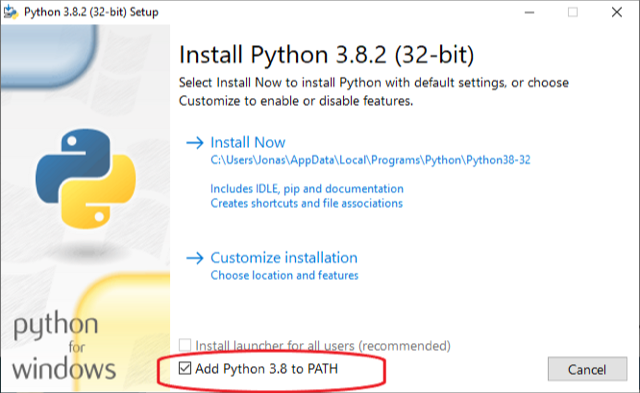
\includegraphics[width=0.8\linewidth,height=0.5\textheight,keepaspectratio]{chapters/06_python1_introduction/figures/python_path.png}
        \end{figure}
    \end{frame}
    
\begin{frame}{Python Interpreter: Windows (II)}
            \textbf{Ausführen des Python-Interpreters:} \\~\
        
Der Python-Interpreter kann auf unterschiedliche Arten geöffnet werden:
        \begin{itemize}
            \item Über das Startmenü \textrightarrow Python3.x
            \item Über die Kommandozeile: 
            \begin{itemize}
                \item{[WIN + R] drücken (oder nach 'Eingabeaufforderung' suchen)}
                \item \code{cmd} eingeben und bestätigen
                \item \code{python} eingeben
            \end{itemize} 
        \end{itemize}
\end{frame}
    
    \begin{frame}{Python Interpreter: Unix (macOS \& Linux)}
        \textbf{Installation:}\\~\
        
        Auf den meisten Unix-Systemen ist bereits eine Python Installation vorhanden. Jedoch handelt es sich dabei i.d.R. um den veralteten Python 2-Interpreter, der nicht mehr unterstützt wird. Daher sollte mind. Python 3.7 installiert werden. \\~\
        Zur Installation des Interpreters muss den Anweisungen des Installationsprogramms gefolgt werden.\\~\
        
        Der Python-Interpreter wird bei der Installation meist automatisch zur Pfad-Variable hinzugefügt. \\~\
        
        \textbf{Ausführen des Python-Interpreters:} \\~\
        
        Der Python-Interpreter kann auf folgende Weise geöffnet werden:
        \begin{itemize}
            \item macOS: Programme \textrightarrow Dienstprogramme \textrightarrow Terminal \textrightarrow \code{python3} eingeben
            \item Linux: Terminal öffnen \textrightarrow \code{python3} eingeben
        \end{itemize}
    \end{frame}
    
    \begin{frame}{Python Interpreter}
        Nachdem der Interpreter geöffnet wurde, sollte folgende (ähnliche) Ausgabe erscheinen:
        
        \begin{figure}
            \centering
            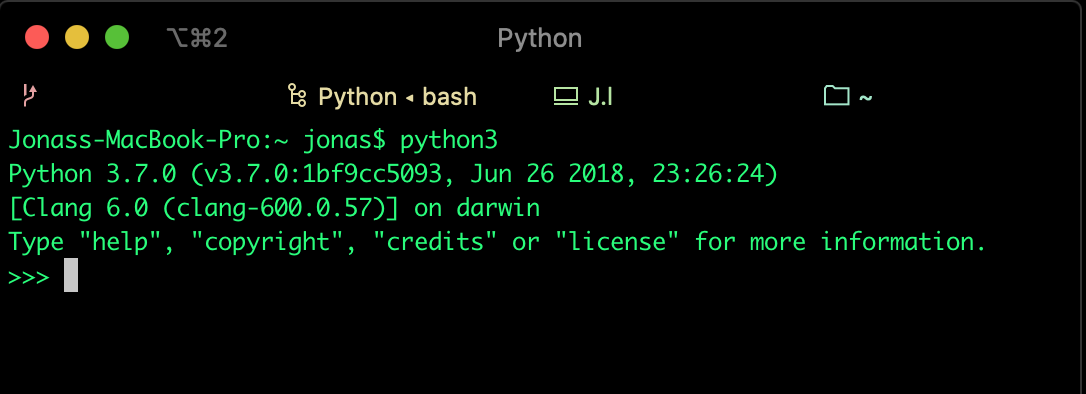
\includegraphics[width=0.8\linewidth,height=0.5\textheight,keepaspectratio]{chapters/06_python1_introduction/figures/interpreter.png}
            \caption{Der Python-Interpreter auf macOS}
        \end{figure}
    \end{frame}
    
    \begin{frame}{Python Interpreter}
        Eine Möglichkeit, Python-Code auszuführen, ist, den Code direkt in die Interpreter-Umgebung einzugeben. Hier wird der Code umgehend ausgeführt und die Ausgabe dem Nutzer angezeigt. \\~\
        
        Dass sich der Nutzer im Interpreter befindet, erkennt er daran, dass die Eingabezeile mit \code{>>>} beginnt. \\~\
        
        Diese Umgebung wird auch als \textbf{REPL} (Read-eval-print loop) bezeichnet, da hier kontinuierlich Befehle vom Nutzer eingelesen, verarbeitet und die Ergebnisse wieder ausgegeben werden. \\~\
        
        Eine weitere Möglichkeit, den Code auszuführen, besteht darin, dem Python-Interpreter den Pfad zu einer Python-Datei zu übergeben. Diese Methode wird später vorgestellt.
    \end{frame}
    
    \begin{frame}[fragile]{Schließen des Interpreters}
        Um den Interpreter-Modus zu beenden und in den normalen Kommandozeilenmodus zurückzukehren (bzw. das Fenster zu schließen, falls der Interpreter nicht über die Kommandozeile geöffnet wurde), gibt es zwei Befehle, die genutzt werden können:
        
\begin{pyconcode}
>>> exit()
\end{pyconcode}

und

\begin{pyconcode}
>>> quit()
\end{pyconcode}
    \end{frame}
    
    
    \begin{subsection}{Aufgaben}
    
        \begin{frame}{Aufgaben}
            \begin{enumerate}
                \item Öffnen Sie den Python-Interpreter. Überprüfen Sie, ob der Python-Interpreter ordnungsgemäß geöffnet wurde. Falls nicht, versuchen Sie das Problem zu lösen.
                
                \item Öffnen Sie den Python-Interpreter und schließen Sie diesen wieder, indem Sie einen Befehl eingeben.
            \end{enumerate}    
        \end{frame}
    
    \end{subsection}